\section{Transformations} 

\textbf{General Equation}

\bigskip
\begin{equationbox}{Transformations}
Let $f(x)$ be a function. Then the function

\[g(x)=a\cdot f(b(x-h))+k\]

is a transformation of $f(x)$ where

\begin{outline}
\1 $a$ is the vertical stretch/compression
\2 If $|a|<1$, then $g$ is a vertical stretch of $f$
\2 If $|a|>1$, then $g$ is a vertical compression of $f$
\2 If $a$ is negative, then $g$ is a reflection of $f$ about the $x-$axis
\1 $b$ is the horizontal stretch
\2 If $|b|<1$, then $g$ is a horizontal stretch of $f$
\2 If $|b|>1$, then $g$ is a horizontal compression of $f$
\2 If $b$ is negative, then $g$ is a reflection of $f$ about the $y-$axis
\1 $h$ is the horizontal shift
\2 If $h>0$, then $g$ is a horizontal shift of $f$ by $h$ units to the right
\2 If $h<0$, then $g$ is a horizontal shift of $f$ by $h$ units to the left
\1 $k$ is the vertical shift
\2 If $k>0$, then $g$ is a vertical shift of $f$ by $k$ units up
\2 If $k<0$, then $g$ is a vertical shift of $f$ by $k$ units down
\end{outline}
\end{equationbox}

\bigskip
\begin{enumerate}[labelindent=*,style=multiline,leftmargin=*,label=\textbf{Example \arabic*:}]
\item Describe the transformation of $f$ by the function $2\cdot g(x)+3=f(x)$.
\vfill\item If $f(3)=-2$, and $g(x)=f(x-2)+3$, what coordinate must be on the graph of $g$?
\vfill\item Let $g(x)=|f(x-1)-2|-3$. What is the vertical shift of $f(x)$ by $g(x)$?
\end{enumerate}

\vfill
\newpage
\begin{multicols*}{2}
\begin{outline}[enumerate]
\medium

\1 If $g(x)=|f(x)|$ and $(-x,y)$ is a coordinate of $f(x)$, which of the following is a coordinate of $g(x)$?

\bigskip
\textbf{Equation/Strategy:} \hrulefill

\bigskip
\textbf{Solve:}

\vfill
\2 $(y,x)$
\2 $(x,y)$
\2 $(x,-y)$
\2 $(-x,y)$
\2 $(-x,-y)$

\midline

\1 The graph of $g(x)$ is shown below.

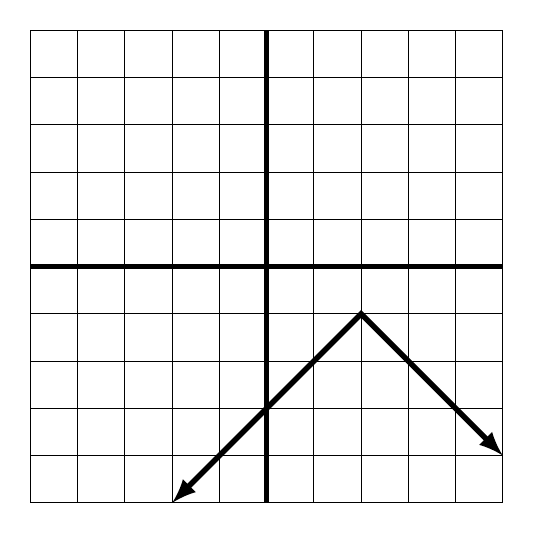
\begin{tikzpicture}[scale=0.6]
\draw (0,0) grid (10,10);
\draw[line width=2pt] (0,5) -- (10,5);
\draw[line width=2pt] (5,0) -- (5,10);
\draw[line width=2pt, latex-latex] (3,0) -- (7,4) -- (10,1);
\end{tikzpicture}

If $g(x)$ is a transformation of $|x|$, which of the following is the equation of $g(x)$?

\bigskip
\textbf{Equation/Strategy:} \hrulefill

\bigskip
\textbf{Solve:}

\vfill
\2 $-|x-2|-1$
\2 $|2-x|-1$
\2 $-|x+2|-1$
\2 $-|x+1|+2$
\2 $-|x-1|+2$

\columnbreak
\advanced

\1 Which of the following can represent a transformation of the function $f(x)$?

\bigskip
\textbf{Equation/Strategy:} \hrulefill

\bigskip
\textbf{Solve:}

\vfill
\2 $\frac{1}{1/f(x)}$
\2 $f(f^{-1}(f(x))$
\2 $\sqrt[3]{f(x)^3}$
\2 $\sqrt{f(x)^2}$
\2 $f(x\cdot0!)$

\midline

\1 The function $f(x)$ has a coordinate $(m,-n)$. $f(x)$ is shifted $k$ units down and $g$ units right, then reflected across the line $y=x$. Which of the following is the resulting coordinate of the transformation?

\bigskip
\textbf{Equation/Strategy:}

\bigskip
\textbf{Solve:}

\vfill
\2 $(-m-g,n+k)$
\2 $(-n+k,m-g)$
\2 $(m-g,-n+k)$
\2 $(-n-k,m-g)$
\2 $(m-g,-n-k)$
\end{outline}
\end{multicols*}